% =============================================================================
%   V. RESULTS
% =============================================================================
\section{Results}
\label{sec:results}

\subsection{RQ1: What the ESG Score Measures}
\label{sec:res_construct}

Little of the ESG schema is filled with ESG data (Table~\ref{tab:provenance}).
The E pillar has four informative indicators: within-sector percentiles of
operating margin, revenue-to-market-value and gross margin, standing in for
emissions, renewable share and waste, and one binary flag for public climate
commitments. Six of the seven S indicators are financial; revenue per
employee even enters twice, once directly and once as a proxy for employee
satisfaction. The G pillar is different, because ISS governance risk scores
fill \ISSShareG\% of its cells.

The consequence is that E and S largely duplicate the financial factors.
Regressing each pillar on the other seven factor scores gives $R^2=\RSqE$
for E and \RSqS for S, against \RSqG for G, and the ESG composite has a
Spearman correlation of \RhoESGFin with the financial score. E and S are
moderately correlated with each other ($\rho=\RhoES$) and nearly unrelated
to G ($\rho=\RhoEG$ and \RhoSG). The label ``ESG'' thus covers two different
objects: a within-sector measure of financial quality (E and S) and largely
independent third-party governance information (G). Conventional diagnostics
miss this. The maximum VIF among factor scores is only \VIFMax
(\VIFMaxFactor), and the first three principal components explain
\PCAFirstThree\% of factor variance, which looks like a well-conditioned
factor set; the redundancy sits inside the ESG block.

The three investor profiles also differ less than their names suggest. The
balanced composite has Spearman correlations of \RhoProfEB and \RhoProfBF
with the ESG-first and financial-first composites, and its top-\TopN list
shares \OverlapEB and \OverlapBF names with them, even though the ESG weight
ranges from \WFinFirstESG\% to \WESGFirstESG\%.

\subsection{RQ2: In-Sample Validation Overstates Quality}
\label{sec:res_insample}

The pipeline's former validation evidence looked strong, and none of it
survives out of sample (Table~\ref{tab:insample}). The balanced composite's
correlation with the trailing six-month return is \InSampleICBalSixM, but
those returns end on the snapshot date and overlap the price history used by
the risk-adjusted and stability factors. Its correlation with the
contemporaneous quality proxy is \InSampleICBalQuality, inflated by inputs
that the proxy shares with the financial, growth and operational factors.
Out of sample, all three profiles have negative point ICs, and every
confidence interval contains zero.

Two further designs inflated the evidence (Table~\ref{tab:prepost}). With
the isotonic correction fitted to the quality proxy, \MonoPre of \MonoTotal
factors were ``monotonic'' in that proxy; without it, \MonoPost are. The
former ``Bayesian bootstrap'' multiplied each score by i.i.d.\
Exponential(1) noise and so measured the injected noise; its rank intervals
had a median width of \PreCIWidthMedian positions out of \PreNFirmsBoot,
while the earlier draft reported perfect rank stability (Kendall $\tau=1$)
from a separate calculation. These problems affected the evidence rather
than the conclusion: the pre-audit composite also has no predictive power
(IC $=\ICPreAuditFull$).

\begin{table}[t]
\centering
\caption{In-sample ``validation'' versus out-of-sample outcome. In-sample
columns are rank correlations of the composite with trailing six-month returns
and with a contemporaneous quality proxy on the snapshot cross-section.
Out-of-sample intervals as in Table~\ref{tab:oos_ic}.}
\label{tab:insample}
\scriptsize
\setlength{\tabcolsep}{3pt}
\resizebox{\columnwidth}{!}{% Auto-generated by scripts/26_paper_artifacts.py
\begin{tabular}{@{}lrrrr@{}}
\toprule
& \multicolumn{2}{c}{In-sample (pre-snapshot)} & \multicolumn{2}{c}{Out-of-sample} \\
\cmidrule(lr){2-3}\cmidrule(l){4-5}
Composite & vs.\ trailing 6m & vs.\ quality proxy & IC, full window & 95\% CI \\
\midrule
Balanced composite & 0.227 & 0.503 & \ensuremath{-}0.094 & [\ensuremath{-}0.227, 0.040] \\
ESG-first composite & 0.093 & 0.272 & \ensuremath{-}0.111 & [\ensuremath{-}0.230, 0.015] \\
Financial-first composite & 0.288 & 0.580 & \ensuremath{-}0.063 & [\ensuremath{-}0.186, 0.073] \\
\bottomrule
\end{tabular}
}
\end{table}

\begin{table}[t]
\centering
\caption{Diagnostics before and after the audit corrections of
Section~\ref{sec:audit}. Pre-audit rank intervals come from the former
``Bayesian bootstrap''; post-audit intervals from Section~\ref{sec:rank_design}.}
\label{tab:prepost}
\scriptsize
% Auto-generated by scripts/26_paper_artifacts.py
\begin{tabular}{@{}p{0.58\columnwidth}rr@{}}
\toprule
Diagnostic & Pre-audit & Post-audit \\
\midrule
Factors monotonic in quintiles of the quality proxy & 7/8 & 3/8 \\
Median 95\% rank-CI width, all firms & 248 & 42 \\
Maximum VIF among factor scores & 2.80 & 2.04 \\
Top-19 balanced portfolio: firms in common & -- & 13/19 \\
Balanced composite: Spearman $\rho$ pre vs.\ post & -- & 0.95 \\
Out-of-sample IC of the balanced composite & \ensuremath{-}0.110 & \ensuremath{-}0.094 \\
\bottomrule
\end{tabular}

\end{table}

\subsection{RQ3: Out-of-Sample Evidence}
\label{sec:res_oos}

Over the window the S\&P~500 returned \IdxRetUS\% and the NIFTY~50
\IdxRetIndia\%, and the equal-weighted mid-cap universes returned
\UnivRetUS\% (US) and \UnivRetIndia\% (India). Table~\ref{tab:primary}
reports the three primary hypotheses.

\begin{table}[t]
\centering
\caption{Primary hypotheses (one-sided tests, Holm-adjusted across H1--H3;
$N=\NOOS$ firms with a full-window return).}
\label{tab:primary}
\scriptsize
\setlength{\tabcolsep}{3pt}
\resizebox{\columnwidth}{!}{% Auto-generated by scripts/26_paper_artifacts.py
\begin{tabular}{@{}llrcrr@{}}
\toprule
& Test & Estimate & 95\% CI & $p$ & $p_{\text{Holm}}$ \\
\midrule
H1 & IC of balanced composite with return & \ensuremath{-}0.094 & [\ensuremath{-}0.219, 0.036] & 0.935 & 1.000 \\
H2 & Partial $\rho$(ESG, realised vol.\,$\mid$\,trailing vol.) & \ensuremath{-}0.163 & [\ensuremath{-}0.276, \ensuremath{-}0.041] & 0.004 & 0.013 \\
H3 & Top-19 minus universe return (pp) & 1.9 & [\ensuremath{-}10.9, 11.5] & 0.543 & 1.000 \\
\bottomrule
\end{tabular}
}
\end{table}

The composite does not predict returns, so H1 and H3 are not supported. Its
IC with the country-neutral full-window return is \HOneEst (95\% CI
$[\HOneLo,\HOneHi]$), and its top-\TopN portfolio beat the universe by
\HThreeEst percentage points (pp), with CI $[\HThreeLo,\HThreeHi]$. The
\NExited firms acquired during the window do not change this. Assigning them
the 5th or 95th percentile return puts the IC in
$[\BoundICLow,\BoundICHigh]$ and the excess return in
$[\BoundExLow,\BoundExHigh]$~pp; the excess turns negative under both bounds
because the top-ranked firm (CTRA) was among the exits and the bounds keep it
in the portfolio.

ESG does predict risk, so H2 is supported. Controlling for trailing
volatility, higher ESG predicts lower realised volatility, with partial
$\rho=\HTwoEst$ (95\% CI $[\HTwoLo,\HTwoHi]$, Holm $p=\HTwoHolm$). The effect
is modest relative to the persistence of volatility itself: trailing
volatility alone has a rank correlation of \RhoVolPersist with realised
volatility, so most of the raw ESG--volatility association
($\rho=\RhoESGVolRaw$) is past volatility carried forward.

The secondary results locate the signal (Figure~\ref{fig:oos_ic} and
Tables~\ref{tab:oos_ic} and~\ref{tab:oos_risk}). No composite has a positive
IC at any horizon, and the only Holm-significant full-window IC is negative,
for the S pillar (\ICSFull). At one month the financial and market scores
have significantly \emph{negative} ICs, consistent with short-term reversal.
In rank regressions with trailing volatility, beta, size, and sector and
country effects, both the composite (\RegVolESG, $p=\RegVolPESG$) and the S
pillar (\RegVolS, $p=\RegVolPS$) predict lower realised volatility, whereas
the E pillar, the G pillar and the part of ESG orthogonal to the other
factors do not. The G pillar's pooled association with realised beta
(\PartBetaG) disappears once sector and country effects are added
(Table~\ref{tab:ext_controls}). The forward risk signal is therefore carried
mainly by the financial-proxy S pillar.

The risk tilt was costly in a rising market (Table~\ref{tab:oos_port}). The
top-\TopN ESG-only portfolio returned \ExESGFull~pp relative to the universe
(CI $[\ExESGFullLo,\ExESGFullHi]$), or \ExESGBA~pp after adjusting for
trailing beta. Sector-and-country neutralisation reduces the gap to
\ExESGSN~pp (CI $[\ExESGSNLo,\ExESGSNHi]$), so more than half of the
shortfall is a sector bet: the portfolio overweights real estate, utilities
and energy and holds no technology or healthcare firms, the two
best-performing sectors of the window.

\begin{figure}[t]
\centering
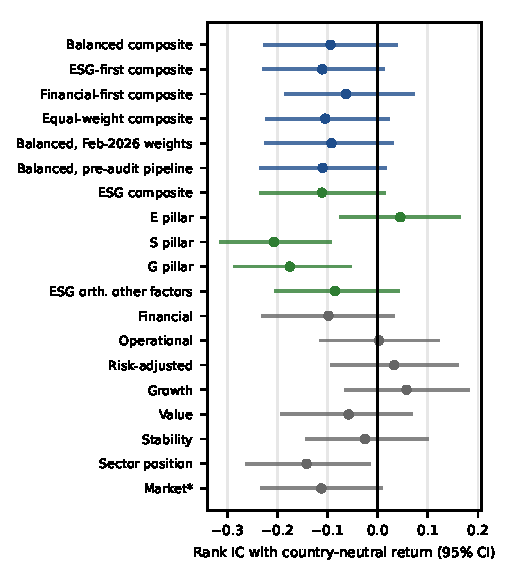
\includegraphics[width=0.95\columnwidth]{fig_oos_ic}
\caption{Out-of-sample rank ICs over (\SnapshotDate,\,\OOSEndDate] with 95\%
bootstrap intervals. Blue: composites; green: ESG measures; grey: financial
factors (*market score carries zero weight). Two-sided 80\%-power detection
threshold: $|\rho|\ge\MDEOOS$.}
\label{fig:oos_ic}
\end{figure}

\begin{table}[t]
\centering
\caption{Out-of-sample rank ICs with country-neutral returns. Bold: Holm
$p<0.05$ within horizon. Intervals use 1,000 resamples, so they differ
slightly from the 5,000-resample H1 interval in Table~\ref{tab:primary}.}
\label{tab:oos_ic}
\scriptsize
\setlength{\tabcolsep}{3pt}
% Auto-generated by scripts/26_paper_artifacts.py
\begin{tabular}{@{}lrrrc@{}}
\toprule
Signal & 1m & 3m & Full & 95\% CI (full) \\
\midrule
ESG composite & \ensuremath{-}0.138 & \ensuremath{-}0.078 & \ensuremath{-}0.111 & [\ensuremath{-}0.235, 0.016] \\
\quad E pillar & \ensuremath{-}0.104 & 0.018 & 0.045 & [\ensuremath{-}0.077, 0.166] \\
\quad S pillar & \ensuremath{-}0.116 & \ensuremath{-}0.164 & \textbf{\ensuremath{-}0.207} & [\ensuremath{-}0.315, \ensuremath{-}0.092] \\
\quad G pillar & \ensuremath{-}0.025 & \ensuremath{-}0.118 & \ensuremath{-}0.175 & [\ensuremath{-}0.288, \ensuremath{-}0.052] \\
ESG $\perp$ other factors & \ensuremath{-}0.054 & \ensuremath{-}0.077 & \ensuremath{-}0.085 & [\ensuremath{-}0.206, 0.045] \\
\midrule
Financial & \textbf{\ensuremath{-}0.190} & \ensuremath{-}0.099 & \ensuremath{-}0.098 & [\ensuremath{-}0.232, 0.034] \\
Operational & \ensuremath{-}0.042 & 0.051 & 0.003 & [\ensuremath{-}0.116, 0.124] \\
Risk-adjusted & \ensuremath{-}0.038 & 0.096 & 0.033 & [\ensuremath{-}0.094, 0.162] \\
Growth & 0.032 & 0.038 & 0.058 & [\ensuremath{-}0.067, 0.182] \\
Value & 0.021 & \ensuremath{-}0.120 & \ensuremath{-}0.058 & [\ensuremath{-}0.193, 0.070] \\
Stability & \ensuremath{-}0.154 & \ensuremath{-}0.076 & \ensuremath{-}0.025 & [\ensuremath{-}0.144, 0.101] \\
Market (not weighted) & \textbf{\ensuremath{-}0.208} & \ensuremath{-}0.073 & \ensuremath{-}0.112 & [\ensuremath{-}0.234, 0.010] \\
Sector position & \ensuremath{-}0.098 & \ensuremath{-}0.074 & \ensuremath{-}0.142 & [\ensuremath{-}0.263, \ensuremath{-}0.013] \\
\midrule
Balanced composite & \ensuremath{-}0.175 & \ensuremath{-}0.074 & \ensuremath{-}0.094 & [\ensuremath{-}0.227, 0.040] \\
ESG-first composite & \ensuremath{-}0.159 & \ensuremath{-}0.082 & \ensuremath{-}0.111 & [\ensuremath{-}0.230, 0.015] \\
Financial-first composite & \ensuremath{-}0.168 & \ensuremath{-}0.051 & \ensuremath{-}0.063 & [\ensuremath{-}0.186, 0.073] \\
Equal-weight composite & \ensuremath{-}0.160 & \ensuremath{-}0.091 & \ensuremath{-}0.105 & [\ensuremath{-}0.224, 0.023] \\
Balanced, Feb-2026 weights & \ensuremath{-}0.171 & \ensuremath{-}0.078 & \ensuremath{-}0.092 & [\ensuremath{-}0.226, 0.032] \\
Balanced, pre-audit pipeline & \textbf{\ensuremath{-}0.189} & \ensuremath{-}0.091 & \ensuremath{-}0.110 & [\ensuremath{-}0.237, 0.017] \\
\bottomrule
\end{tabular}

\end{table}

\begin{table}[t]
\centering
\caption{Top-\TopN portfolio excess return over the equal-weighted universe
(pp, country-neutral). $\beta$-adj.: market-model adjustment with trailing
beta; Sect.-neut.: sector-and-country-neutral full-window returns.}
\label{tab:oos_port}
\scriptsize
\setlength{\tabcolsep}{2.5pt}
\resizebox{\columnwidth}{!}{% Auto-generated by scripts/26_paper_artifacts.py
\begin{tabular}{@{}lrrrrrc@{}}
\toprule
Top-$N$ by & 1m & 3m & Full & $\beta$-adj. & Sect.-neut. & 95\% CI (full) \\
\midrule
Balanced composite & 2.2 & 0.9 & 1.9 & 1.6 & 3.1 & [\ensuremath{-}11.2, 11.0] \\
ESG-first composite & \ensuremath{-}0.6 & \ensuremath{-}5.7 & \ensuremath{-}9.4 & \ensuremath{-}8.6 & \ensuremath{-}0.8 & [\ensuremath{-}18.5, 0.8] \\
Financial-first composite & 1.5 & 2.5 & 0.9 & 0.3 & \ensuremath{-}1.3 & [\ensuremath{-}10.5, 13.8] \\
Equal-weight composite & 0.3 & \ensuremath{-}0.9 & \ensuremath{-}2.8 & \ensuremath{-}3.8 & 1.0 & [\ensuremath{-}11.4, 7.7] \\
Balanced, Feb-2026 weights & 0.5 & \ensuremath{-}1.0 & 2.1 & 1.3 & 6.4 & [\ensuremath{-}9.7, 16.2] \\
Balanced, pre-audit pipeline & 1.2 & \ensuremath{-}2.3 & \ensuremath{-}3.4 & \ensuremath{-}3.2 & \ensuremath{-}2.8 & [\ensuremath{-}12.6, 4.9] \\
ESG composite & \ensuremath{-}1.1 & \ensuremath{-}8.0 & \ensuremath{-}19.9 & \ensuremath{-}17.4 & \ensuremath{-}8.4 & [\ensuremath{-}27.9, \ensuremath{-}10.2] \\
\bottomrule
\end{tabular}
}
\end{table}

\begin{table}[t]
\centering
\caption{ESG and realised risk. Partial $\rho$ controls for the trailing value
of the same risk measure; bold: Holm $p<0.05$ across the 15 secondary tests.
Regression: rank of realised volatility on ESG rank with trailing volatility,
beta, size, and sector and country effects (HC3).}
\label{tab:oos_risk}
\scriptsize
\setlength{\tabcolsep}{2.5pt}
\resizebox{\columnwidth}{!}{% Auto-generated by scripts/26_paper_artifacts.py
\begin{tabular}{@{}lrrrrr@{}}
\toprule
& \multicolumn{2}{c}{Realised volatility} & Realised $\beta$ & \multicolumn{2}{c}{Vol.\ regression} \\
\cmidrule(lr){2-3}\cmidrule(lr){4-4}\cmidrule(l){5-6}
ESG measure & raw $\rho$ & partial $\rho$ & partial $\rho$ & coef. & $p$ \\
\midrule
ESG composite & \ensuremath{-}0.303 & \ensuremath{-}0.163 & \textbf{\ensuremath{-}0.239} & \ensuremath{-}0.085 & 0.019 \\
\quad E pillar & \ensuremath{-}0.151 & \ensuremath{-}0.071 & \ensuremath{-}0.067 & \ensuremath{-}0.052 & 0.142 \\
\quad S pillar & \ensuremath{-}0.285 & \ensuremath{-}0.123 & \textbf{\ensuremath{-}0.330} & \ensuremath{-}0.103 & 0.014 \\
\quad G pillar & \ensuremath{-}0.252 & \ensuremath{-}0.125 & \textbf{\ensuremath{-}0.238} & 0.005 & 0.908 \\
ESG $\perp$ other factors & \ensuremath{-}0.184 & \ensuremath{-}0.154 & \ensuremath{-}0.071 & \ensuremath{-}0.056 & 0.093 \\
\bottomrule
\end{tabular}
}
\end{table}

\subsection{RQ4: Where the Risk Signal Comes From}
\label{sec:res_mechanism}

Because H2 is the only supported hypothesis, we test it against the three
alternative explanations of Section~\ref{sec:ext_design}
(Figure~\ref{fig:mechanism}, Tables~\ref{tab:ext_controls}
and~\ref{tab:ext_robust}).

\begin{figure*}[t]
\centering
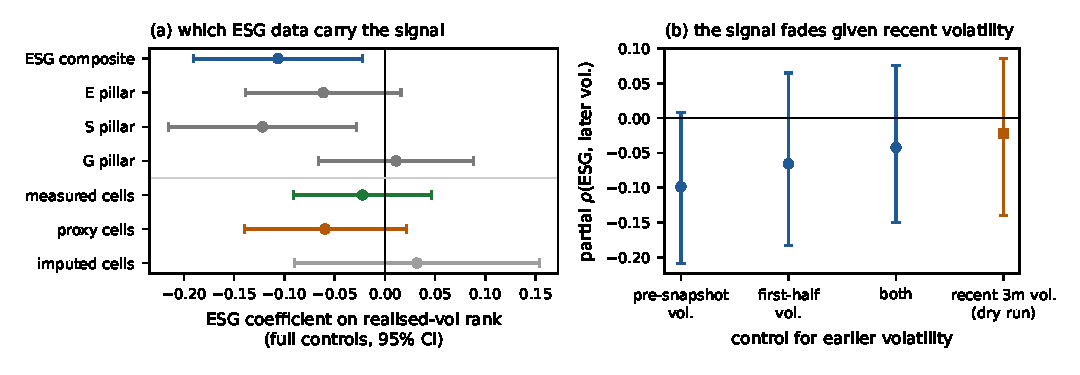
\includegraphics[width=0.92\textwidth]{fig_ext_mechanism}
\caption{Where the ESG risk signal comes from. (a) Coefficient of each ESG
measure in a rank regression of realised OOS volatility with all
\NControls controls and sector and country fixed effects. (b) Partial
Spearman correlation of ESG with realised volatility after \SplitDate, given
earlier volatility. The orange point is the registered dry run: volatility
over (\DryAnchor,\,\DryEnd] given the preceding months. 95\% intervals.}
\label{fig:mechanism}
\end{figure*}

The signal survives known risk characteristics. With all controls and
sector and country effects, the ESG coefficient is \HFourEst (95\% CI
$[\HFourLo,\HFourHi]$, one-sided $p=\HFourP$; H4). A double sort agrees:
within trailing-volatility terciles, high-ESG firms had \DSAvg~pp lower
realised volatility than low-ESG firms on average (CI $[\DSLo,\DSHi]$), and
the gap widens from \DSLowTerc~pp in the calmest tercile to \DSHighTerc~pp in
the most volatile. The result holds without the \NPinned takeover-pinned
firms, with winsorised volatility and without utilities and real estate, and
it has the same sign in both countries (US \HTwoUS, India \HTwoIndia). The
ESG--beta association does not survive full controls (\BetaFullESG,
$p=\BetaFullESGP$), and no ESG measure predicts drawdowns.

The signal does not come from measured ESG data. It sits in the S pillar
(\HFourS, $p=\HFourSP$), whose inputs are almost all financial proxies,
while the G pillar carries none of it (\HFourG). Splitting each firm's cells
by source makes the point directly. Measured cells (ISS, SEC, registry) are
nearly independent of the financial factors ($R^2=\RSqMeas$) and have
partial $\rho=\PartMeas$ with realised volatility (CI
$[\PartMeasLo,\PartMeasHi]$). Proxy cells are largely financial
($R^2=\RSqProxy$) and have the same sign as the S pillar, though imprecisely
($\rho=\PartProxy$, CI $[\PartProxyLo,\PartProxyHi]$). Imputed cells show a
strong raw association (\PartImp) that vanishes once sector fixed effects
are included. Adding measured-cell ESG to the out-of-fold volatility
forecast changes $R^2$ by \CVDeltaMeas.

The signal is small and partly stale volatility. Adding the composite to a
cross-validated volatility forecast raises out-of-fold $R^2$ from \CVBaseRSq
to \CVESGRSq, an improvement in \CVShareImproved\% of repeats but only
\CVDeltaESG in size. Given pre-snapshot volatility, ESG's partial
correlation with second-half volatility is \RecTrail; given first-half
realised volatility, which an investor would have observed, it falls to
\RecFirst (CI $[\RecFirstLo,\RecFirstHi]$, $p=\RecFirstP$). The monthly
partial correlations are negative in \MonNegPartial of \NMonths months but
small. ESG therefore behaves like a slow-moving summary of a firm's risk
profile, adding a little beyond long-horizon trailing volatility and little
beyond recent volatility.

\begin{table}[t]
\centering
\caption{Rank-regression coefficients of each ESG measure for realised risk.
``Trailing'': control for the pre-snapshot value of the same risk measure;
``full'': all controls of Section~\ref{sec:ext_design}, with sector and
country fixed effects (HC3). Drawdown is signed, so a positive value means a
shallower drawdown. Bold: $p<0.05$ (two-sided, unadjusted). $N=\NOOS$.}
\label{tab:ext_controls}
\scriptsize
\setlength{\tabcolsep}{3pt}
\resizebox{\columnwidth}{!}{% Auto-generated by scripts/26_paper_artifacts.py
\begin{tabular}{@{}lrrrrr@{}}
\toprule
& \multicolumn{2}{c}{Realised vol.} & \multicolumn{2}{c}{Realised $\beta$} & Drawdown \\
\cmidrule(lr){2-3}\cmidrule(lr){4-5}\cmidrule(l){6-6}
ESG measure & trailing & full & trailing & full & full \\
\midrule
ESG composite & \textbf{\ensuremath{-}0.087} & \textbf{\ensuremath{-}0.106} & \textbf{\ensuremath{-}0.138} & \ensuremath{-}0.033 & 0.060 \\
\quad E pillar & \ensuremath{-}0.048 & \ensuremath{-}0.061 & \textbf{\ensuremath{-}0.103} & 0.000 & 0.063 \\
\quad S pillar & \textbf{\ensuremath{-}0.103} & \textbf{\ensuremath{-}0.122} & \textbf{\ensuremath{-}0.114} & 0.035 & 0.089 \\
\quad G pillar & \ensuremath{-}0.001 & 0.011 & \ensuremath{-}0.055 & \ensuremath{-}0.043 & \ensuremath{-}0.088 \\
\midrule
Measured-cell ESG & \ensuremath{-}0.018 & \ensuremath{-}0.022 & \ensuremath{-}0.064 & \ensuremath{-}0.021 & \ensuremath{-}0.069 \\
Proxy-cell ESG & \ensuremath{-}0.067 & \ensuremath{-}0.059 & \textbf{\ensuremath{-}0.144} & 0.048 & 0.071 \\
Imputed-cell ESG & 0.025 & 0.032 & 0.047 & \ensuremath{-}0.056 & 0.094 \\
\bottomrule
\end{tabular}
}
\end{table}

\begin{table}[t]
\centering
\caption{Robustness of the ESG--volatility result. Upper panel: H2 and H4 on
subsamples. Lower panel: partial Spearman correlation of ESG with realised
volatility after \SplitDate, given earlier volatility.}
\label{tab:ext_robust}
\scriptsize
\setlength{\tabcolsep}{2.5pt}
\resizebox{\columnwidth}{!}{% Auto-generated by scripts/26_paper_artifacts.py
\begin{tabular}{@{}lrcc@{}}
\toprule
Sample / test & $N$ & H2 partial $\rho$ [95\% CI] & H4 coef.\ [95\% CI] \\
\midrule
all (pre-declared) & 260 & \ensuremath{-}0.163 [\ensuremath{-}0.27, \ensuremath{-}0.04] & \ensuremath{-}0.106 [\ensuremath{-}0.19, \ensuremath{-}0.02] \\
excl. deal-pinned & 258 & \ensuremath{-}0.166 [\ensuremath{-}0.27, \ensuremath{-}0.04] & \ensuremath{-}0.104 [\ensuremath{-}0.18, \ensuremath{-}0.03] \\
winsorised vol 1/99 & 260 & \ensuremath{-}0.163 [\ensuremath{-}0.27, \ensuremath{-}0.05] & \ensuremath{-}0.106 [\ensuremath{-}0.19, \ensuremath{-}0.02] \\
US only & 172 & \ensuremath{-}0.208 [\ensuremath{-}0.35, \ensuremath{-}0.06] & \ensuremath{-}0.067 [\ensuremath{-}0.17, 0.04] \\
India only & 88 & \ensuremath{-}0.267 [\ensuremath{-}0.46, \ensuremath{-}0.04] & \ensuremath{-}0.174 [\ensuremath{-}0.41, 0.06] \\
excl. Utilities, Real Estate & 233 & \ensuremath{-}0.171 [\ensuremath{-}0.29, \ensuremath{-}0.04] & \ensuremath{-}0.110 [\ensuremath{-}0.20, \ensuremath{-}0.02] \\
\midrule
2nd-half vol.\ $\mid$ pre-snapshot vol. & 260 & \ensuremath{-}0.099 [\ensuremath{-}0.21, 0.01] & -- \\
2nd-half vol.\ $\mid$ 1st-half vol. & 260 & \ensuremath{-}0.066 [\ensuremath{-}0.18, 0.06] & -- \\
2nd-half vol.\ $\mid$ both & 260 & \ensuremath{-}0.042 [\ensuremath{-}0.15, 0.08] & -- \\
\bottomrule
\end{tabular}
}
\end{table}

\subsection{Robustness of the Return Null}
\label{sec:res_null}

The failure of H1 does not depend on the chosen weights
(Figure~\ref{fig:ext_weights}). Across \WDraws weight vectors drawn uniformly
from the simplex, the OOS IC has median \WICMedian and is positive in only
\WSharePos\% of draws. More ESG weight lowers the IC, which moves from
\SweepICZero with no ESG to \SweepICOne with ESG only. The low risk of the
index portfolio does not come from ESG either: its realised volatility is
below the universe's in \WShareLowVol\% of draws whatever the ESG weight, and
already \SweepVolZero~pp relative to the universe with no ESG weight, because
the risk-adjusted and stability factors select calm firms. Monthly ICs of the
balanced composite are negative in \MonNegICBal of \NMonths months, and
round-trip costs of \CostRT~pp leave a net excess of \NetExBase~pp
(\NetExStress~pp at three times the costs), which does not change the H3
conclusion.

\begin{figure*}[t]
\centering
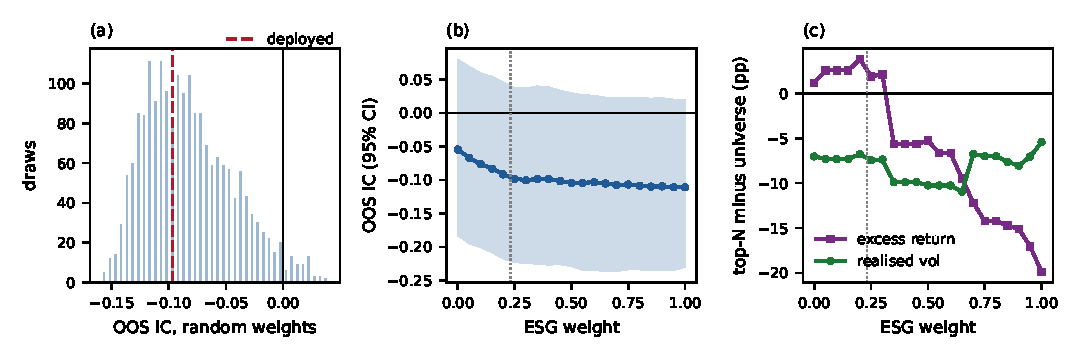
\includegraphics[width=0.9\textwidth]{fig_ext_weights}
\caption{Weight uncertainty and the ESG weight. (a) OOS IC of the composite
under \WDraws weight vectors drawn uniformly from the simplex; dashed line:
deployed weights. (b) OOS IC as the ESG weight rises from 0 to 1, with the
other weights in their deployed proportions (95\% bootstrap band). (c) The
top-\TopN portfolio's excess return and realised volatility relative to the
universe on the same sweep. Dotted line: deployed ESG weight.}
\label{fig:ext_weights}
\end{figure*}

\subsection{Rank Uncertainty}
\label{sec:res_rank}

Given the construction, rankings near the top are reasonably well determined
(Figure~\ref{fig:rank_ci} and Table~\ref{tab:top}). For the top-\TopN names,
the median 95\% rank interval spans \CIWidthTop ranks, and weight
uncertainty dominates sampling uncertainty (\CIWidthTopWeights against
\CIWidthTopSampling ranks). Of the \TopN current constituents, \NPTopHalf
remain in the top-\TopN in at least half of the draws, and a perturbed
portfolio is expected to share \ExpOverlap names with the published one.
Stable rankings do not, however, make the construction predictive.

\begin{figure}[t]
\centering
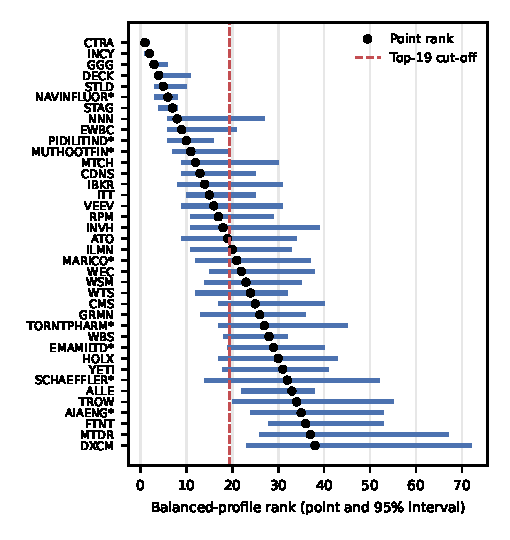
\includegraphics[width=0.9\columnwidth]{fig_rank_ci}
\caption{Balanced-profile ranks with 95\% intervals combining universe
resampling and Dirichlet ($\kappa=\BootKappa$) weight perturbation
($B=\BootN$). *NSE-listed.}
\label{fig:rank_ci}
\end{figure}

\begin{table}[t]
\centering
\caption{Top-\TopN balanced portfolio: 95\% rank interval, probability of
remaining in the top-\TopN, and realised full-window return ($^\dagger$NSE;
``exit'': acquired during the window).}
\label{tab:top}
\scriptsize
\setlength{\tabcolsep}{2.5pt}
\resizebox{\columnwidth}{!}{% Auto-generated by scripts/26_paper_artifacts.py
\begin{tabular}{@{}rllrr r@{}}
\toprule
Rank & Ticker & Sector & 95\% CI & $P(\text{top-}N)$ & OOS ret.\ (\%) \\
\midrule
1 & CTRA & Energy & [1, 2] & 1.00 & exit \\
2 & INCY & Healthcare & [1, 2] & 1.00 & 29.9 \\
3 & GGG & Industrials & [3, 6] & 1.00 & \ensuremath{-}6.7 \\
4 & DECK & Consumer Cyclical & [3, 11] & 1.00 & \ensuremath{-}20.1 \\
5 & STLD & Basic Materials & [3, 10] & 1.00 & 30.3 \\
6 & NAVINFLUOR$^{\dagger}$ & Basic Materials & [3, 8] & 1.00 & 43.7 \\
7 & STAG & Real Estate & [4, 8] & 1.00 & 1.8 \\
8 & NNN & Real Estate & [6, 27] & 0.93 & \ensuremath{-}0.7 \\
9 & EWBC & Financial Services & [6, 21] & 0.96 & 15.7 \\
10 & PIDILITIND$^{\dagger}$ & Basic Materials & [6, 16] & 1.00 & 25.6 \\
11 & MUTHOOTFIN$^{\dagger}$ & Financial Services & [7, 19] & 0.99 & \ensuremath{-}9.4 \\
12 & MTCH & Communication Services & [9, 30] & 0.68 & 30.3 \\
13 & CDNS & Technology & [9, 25] & 0.87 & 10.9 \\
14 & IBKR & Financial Services & [8, 31] & 0.76 & 35.4 \\
15 & ITT & Industrials & [10, 25] & 0.84 & 10.1 \\
16 & VEEV & Healthcare & [9, 31] & 0.73 & 55.6 \\
17 & RPM & Basic Materials & [11, 29] & 0.52 & 3.2 \\
18 & INVH & Real Estate & [11, 39] & 0.42 & 6.5 \\
19 & ATO & Utilities & [9, 34] & 0.60 & \ensuremath{-}16.4 \\
\bottomrule
\end{tabular}
}
\end{table}
